%%%%%%%%%%%%%%%%%%%%%%%%%%%%%%%%%%%%%%%%%%%%%%%%%%%%%%%%%%%%%%%%%%%%%%
% Lớp 10 | Hệ thức lượng trong tam giác | Định lý sin và định lý côsin
% Dạng 0H4?2-2: Bài toán có dùng công thức diện tích
% Số câu: 52  (sinh tự động bởi tach_cau.py; từ nay thầy sửa trực tiếp file này)
%%%%%%%%%%%%%%%%%%%%%%%%%%%%%%%%%%%%%%%%%%%%%%%%%%%%%%%%%%%%%%%%%%%%%%

%%%%%%%%%%%%%%%% TRẮC NGHIỆM 4 PHƯƠNG ÁN %%%%%%%%%%%%%%%%

% nguồn: MaHoaNH_TracNghiem_Lop10
\begin{ex}%[0H4N2-2]%[ma:f3b330d0]
	Cho tam giác $ABC$ có $AB=c$, $AC=b$, $CB=a$, $p=\dfrac{a+b+c}{2}$.  Diện tích $S$ của tam giác $ABC$ được tính theo công thức nào sau đây?
	\choice {$S=\sqrt{p(p+a)(p+b)(p+c)}$}{$S=\dfrac{1}{2}ac\cos  A$}{$S=bc\cos A$}{\True $S=\sqrt{p(p-a)(p-b)(p-c)}$}
	\loigiai{ 
		Công thức tính diện tích $S$ của tam giác khi biết ba cạnh  (Công thức Heron) là $$S=\sqrt{p(p-a)(p-b)(p-c)}.$$
	 }
\end{ex}

% nguồn: MaHoaNH_TracNghiem_Lop10
\begin{ex}%[0H4N2-2]%[ma:7a9674d1]
	Cho tam giác $ABC$ có $AB=c$, $AC=b$ và góc $A$. Diện tích $S$ của tam giác  $ABC$ được tính theo công thức nào sau đây?
	\choice {$S=bc\sin A$}{$S=\dfrac{1}{2}bc\cos A$}{$S=bc\cos A$}{\True $S=\dfrac{1}{2}bc\sin A$} 
	 \loigiai{
		Công thức  tính diện tích tam giác khi biết hai cạnh $b, c$ và góc xen giữa $A$ là $S=\dfrac{1}{2}b c \sin A$.
	} 
\end{ex}

% nguồn: MaHoaNH_TracNghiem_Lop10
\begin{ex}%[0H4N2-2]%[ma:95e3b5d7]
	Cho tam giác $ABC$ có $a=4$, $c=5$, $\widehat{B}=150^\circ$. Tính diện tích $S$ của tam giác $ABC$. 
	\choice 
		{$S=10$} 
		 {$S=10\sqrt{3}$}
		{\True  $S=5$}
		 {$S=5\sqrt{3}$}
	 \loigiai{
	Diện tích tam giác $ABC$ là $S=\dfrac{1}{2}ac\sin \widehat{B}=\dfrac{1}{2}\cdot 4\cdot 5\sin 150^\circ =5$.} 
\end{ex}

% nguồn: MaHoaNH_TracNghiem_Lop10
\begin{ex}%[0H4N2-2]%[ma:b7fbb20c]
	Cho $\triangle ABC$ có $a=2$, $b=6$, $\widehat{C}=135^\circ$. Diện tích của tam giác là 
	\choice 
		 {$4$}
		 {$6\sqrt{2}$}
		{\True  $3\sqrt{2}$}
		{$4\sqrt{2}$} 
	\loigiai{ 
	Ta có $S_{\triangle ABC}=\dfrac{1}{2}a\cdot  b\cdot\sin C=\dfrac{1}{2}\cdot 2\cdot 6\cdot\sin{135^\circ}=3\sqrt{2}$.}
\end{ex}

% nguồn: MaHoaNH_TracNghiem_Lop10
\begin{ex}%[0H4N2-2]%[ma:97776ef7]
	Cho tam giác $ABC$  có $\widehat{A}=60^\circ$, $b=10$, $c=20$. Diện tích tam giác $ABC$ bằng
	 \choice
		{$70\sqrt{3}$} 
		 {$60\sqrt{3}$}
		{\True  $50\sqrt{3}$}
		{$40\sqrt{3}$} 
	\loigiai{ 
	Ta có $S_{\triangle  ABC}=\dfrac{1}{2}b\cdot c\cdot \sin \widehat{A}=\dfrac{1}{2}\cdot 10\cdot 20\cdot \sin 60^\circ =50\sqrt{3}$.}
\end{ex}

% nguồn: MaHoaNH_TracNghiem_Lop10
\begin{ex}%[0H4N2-2]%[ma:208fabf1]
	Tam giác  có độ dài ba cạnh lần lượt là $9$, $10$, $11$ có diện tích bằng
	\choice 
		 {$15\sqrt{2}$}
		{\True $30\sqrt{2}$} 
		{$50\sqrt{3}$} 
		 {$25\sqrt{3}$}
	\loigiai{ 
		Nửa chu  vi của tam giác đã cho là $p=\dfrac{9+10+11}{2}=15$.\\
	Diện tích của tam giác đã cho là $S=\sqrt{p\left(p-9\right)\left(p-10\right)\left(p-11\right)}=30\sqrt{2}$.} 
\end{ex}

% nguồn: MaHoaNH_TracNghiem_Lop10
\begin{ex}%[0H4N2-2]%[ma:79fe2991]
	Cho tam giác $ABC$ có $AB=3$, $AC=7$, $BC=8$. Tính  diện tích tam giác $ABC$.
	 \choice
		{$S=5\sqrt{3}$} 
		{\True  $S=6\sqrt{3}$}
		 {$S=4\sqrt{3}$}
		 {$S=3\sqrt{3}$}
	 \loigiai{
		Áp dụng công thức Hê-rông  ta có $S=\sqrt{p(p-a)(p-b)(p-c)}=6\sqrt{3}$.
	 }
\end{ex}

% nguồn: MaHoaNH_TracNghiem_Lop10
\begin{ex}%[0H4H2-2]%[ma:6d95a0ac]
	Cho $\triangle ABC$ có $b=7$; $c=5$; $\cos A=\dfrac{3}{5}$. Độ  dài đường cao $h_a$ của tam giác $\triangle ABC$ là
	\choice 
		 {\True $\dfrac{7\sqrt{2}}{2}$}
		 {$8$}
		{$8\sqrt{3}$} 
		{$80\sqrt{3}$} 
	\loigiai{ 
		Ta có $a=\sqrt{b^2+c^2-2bc\cos  A}=\sqrt{7^2+5^2-2\cdot 7\cdot 5\cdot\dfrac{3}{5}}=\sqrt{32}=4\sqrt{2}$.\\
		Vì $0 < \widehat{A} <  180^\circ$ nên $\sin A=\sqrt{1-\cos^2A}=\sqrt{1-\left(\dfrac{3}{5}\right)^2}=\dfrac{4}{5}$.\\
	$S=\dfrac{1}{2}bc\sin A=\dfrac{1}{2}\cdot 7\cdot 5\cdot\dfrac{4}{5}=14$ mà $S=\dfrac{1}{2}a\cdot h_a\Leftrightarrow 14=\dfrac{1}{2}\cdot 4\sqrt{2}\cdot h_a\Leftrightarrow  h_a=\dfrac{7\sqrt{2}}{2}$.}
\end{ex}

% nguồn: MaHoaNH_TracNghiem_Lop10
\begin{ex}%[0H4H2-2]%[ma:c426294d]
	Cho tam  giác $ABC$ có góc $\widehat A=30^\circ$, góc $\widehat B=45^\circ$. Tính $\dfrac{h_a}{h_b}$.
	\choice 
		{$\dfrac{h_a}{h_b}=\dfrac{1}{2}$} 
		{$\dfrac{h_a}{h_b}=\dfrac{1}{2\sqrt 2}$} 
		{\True  $\dfrac{h_a}{h_b}=\sqrt 2 $}
		 {$\dfrac{h_a}{h_b}=\dfrac{\sqrt 2}{2}$}
	\loigiai{ 
		Ta có $S=\dfrac{1}{2}a\cdot h_a=\dfrac{1}{2}b\cdot  h_b\Rightarrow\dfrac{h_a}{h_b}=\dfrac{b}{a}$.\\
		Theo định lý sin có $\dfrac{a}{\sin A}=\dfrac{b}{\sin B}\Rightarrow\dfrac{b}{a}=\dfrac{\sin B}{\sin A}=\dfrac{\sin{45^\circ}}{\sin{30^\circ}}=\dfrac{\dfrac{1}{\sqrt  2}}{\dfrac{1}{2}}=\sqrt 2 $.\\
		Vậy $\dfrac{h_a}{h_b}=\dfrac{b}{a}=\sqrt 2 $. 
	 }
\end{ex}

% nguồn: MaHoaNH_TracNghiem_Lop10
\begin{ex}%[0H4Y2-2]%[ma:c8f4b5c0]
	Trong mặt phẳng $O x y$, phương trình đường tròn tâm $I(3;-1)$, bán kính $R=25$ là 
	 \choice
		{$(x-3)^2+(y+1)^2=25$} 
		{$(x+3)^2+(y-1)^2=625$} 
		{$(x-3)^2+(y+1)^2=5$} 
		{\True$(x-3)^2+(y+1)^2=625$} 
	\loigiai{Phương trình đường tròn tâm  $I(3;-1)$, bán kính $R=25$ là $(x-3)^2+(y+1)^2=25^2$}
\end{ex}

% nguồn: MaHoaNH_TracNghiem_Lop10
\begin{ex}%[0H4B2-2]%[ma:5b7506e9]
	Phương trình đường tròn $\left(C\right)$ có tâm $I\left(-1;2\right)$  và đi qua điểm $M\left(3;5\right)$ là?
	 \choice
		{$\left(x+1\right)^2+\left(y-2\right)^2=5$} 
		{\True $\left(x+1\right)^2+\left(y-2\right)^2=25$} 
		{$\left(x-1\right)^2+\left(y+2\right)^2=25$} 
		{$\left(x+1\right)^2+\left(y+2\right)^2=25$} 
	\loigiai{Đường tròn $\left(C\right)$ có tâm $I\left(-1;2\right)$ và đi qua điểm $M\left(3;5\right)$ nên $R=IM=5$.  Vậy phương trình đường tròn là$\colon\left(x+1\right)^2+\left(y-2\right)^2=25$
	 }
\end{ex}

% nguồn: MaHoaNH_TracNghiem_Lop10
\begin{ex}%[0H4Y2-2]%[ma:e52f718c]
	Trong  mặt phẳng tọa độ $Oxy$, tìm phương trình của đường tròn có tâm $I(-3; 2)$ và bán kính $R=2$.
	\choice 
		{$(x-3)^2+(y+2)^2=5$} 
		 {\True $(x+3)^2+(y-2)^2=4$}
		 {$(x+3)^2+(y-2)^2=2$}
		{$(x-3)^2+(y+2)^2=4$} 
	\loigiai{Phương trình  của đường tròn có tâm $I(-3; 2)$ và bán kính $R=2$ là $(x+3)^2+(y-2)^2=4$.
	 }
\end{ex}

% nguồn: MaHoaNH_TracNghiem_Lop10
\begin{ex}%[0H4Y2-2]%[ma:865f61cf]
	Trong  mặt phẳng tọa độ $Oxy$, cho đường tròn $(C)\colon x^2+y^2-2x-2y-2=0$. Điểm nào sau đây thuộc đường tròn $(C)$?
	 \choice
		 {$M(1;0)$}
		 {\True $N(1;3)$}
		 {$Q(2;2)$}
		 {$P(3;-1)$}
	 \loigiai{
		Tọa độ điểm $N(1;3)$  thỏa mãn phương trình đường tròn $(C)$. Do đó, $N\in (C)$.
	} 
\end{ex}

% nguồn: MaHoaNH_TracNghiem_Lop10
\begin{ex}%[0H4Y2-2]%[ma:daa9d622]
	Trong mặt phẳng  toạ độ $Oxy$, phương trình đường tròn có tâm $I(-2; 1)$ và bán kính $R=2$ là
	\choice 
		 {$(x+2)^2+(y-1)^2=2$}
		{\True $(x+2)^2+(y-1)^2=4$} 
		 {$(x-2)^2+(y+1)^2=2$}
		 {$(x-2)^2+(y+1)^2=4$}
	 \loigiai{
		Phương trình đường tròn có tâm  $I(-2; 1)$ và bán kính $R=2$ là $(x+2)^2+(y-1)^2=4$.
	 }
\end{ex}

% nguồn: MaHoaNH_TracNghiem_Lop10
\begin{ex}%[0H4B2-2]%[ma:2cf7a424]
	Phương  trình đường tròn có tâm $I(-2; 4)$ và bán kính $R = 5$ là
	 \choice
		{$(x-2)^2+(y+4)^2=5$} 
		 {$(x+2)^2+(y-5)^2=25$}
		{\True $(x+2)^2+(y-4)^2=25$} 
		 {$(x-2)^2+(y+4)^2=25$}
	\loigiai{ 
		Phương trình đường  tròn có tâm $I(-2; 4)$ và bán kính $R = 5$ là $(x+2)^2+(y-4)^2=25$.
	 }
\end{ex}

% nguồn: MaHoaNH_TracNghiem_Lop10
\begin{ex}%[0H4Y2-2]%[ma:69a80f9a]
	Viết phương trình đường tròn tâm $I(2;  3)$, bán kính $R=2$.
	\choice 
		 {$(x+2)^2+(y+3)^2=2$}
		{\True $(x-2)^2+(y-3)^2=4$} 
		{$(x+2)^2+(y+3)^2=4$} 
		{$(x-2)^2+(y-3)^2=2$} 
	 \loigiai{
		Phương trình đường tròn tâm  $I(2; 3)$, bán kính $R=2$ là $$(x-2)^2+(y-3)^2=2^2\Leftrightarrow (x-2)^2+(y-3)^2=4.$$
	} 
\end{ex}

% nguồn: MaHoaNH_TracNghiem_Lop10
\begin{ex}%[0H4Y2-2]%[ma:95166a92]
	Phương trình đường tròn $\left(C\right)$ có  tâm $I\left(1;2\right)$ và bán kính $R=6$ là
	\choice 
		{$\left(x-1\right)^2+\left(y-2\right)^2=6$} 
		{$\left(x+1\right)^2+\left(y+2\right)^2=6$} 
		 {$\left(x+1\right)^2+\left(y+2\right)^2=36$}
		{\True  $\left(x-1\right)^2+\left(y-2\right)^2=36$}
	\loigiai{ 
		Phương trình đường tròn $\left(C\right)$ có tâm $I\left(1;2\right)$ và bán kính $R=6$ là  $\left(x-1\right)^2+\left(y-2\right)^2=36$.
	} 
\end{ex}

% nguồn: MaHoaNH_TracNghiem_Lop10
\begin{ex}%[0H4Y2-2]%[ma:c1596c6f]
	Phương trình nào sau đây  là phương trình đường tròn?
	 \choice
		 {\True $x^2+y^2-x=0$}
		 {$x^2-y^2-2 x+2 y-1=0$}
		{$x^2+y^2+2  x y-1=0$}
		{$x^2+y^2-x-y+9=0$} 
	\loigiai{ 
		Phương  trình $x^2+y^2-x=0$ là phương trình đường tròn vì $ a^2+b^2-c>0 $.
	 }
\end{ex}

% nguồn: MaHoaNH_TracNghiem_Lop10
\begin{ex}%[0H4Y2-2]%[ma:c52efa0a]
	Phương trình chính tắc  của đường tròn tâm $I(a;b)$, bán kính $R$ là
	 \choice
		{\True  $(x-a)^2+(y-b)^2=R^2$}
		{$(x+a)^2+(y+b)^2=R^2$} 
		 {$\left(x_0-a\right)(x-a)+\left(y_0-b\right)(y-b)=R^2$}
		{$(x-a)^2+(y-b)^2=R$} 
	\loigiai{ 
		Phương trình chính tắc của  đường tròn tâm $I(a;b)$, bán kính $R$ là $(x-a)^2+(y-b)^2=R^2$.
	} 
\end{ex}

% nguồn: MaHoaNH_TracNghiem_Lop10
\begin{ex}%[0H4Y2-2]%[ma:f4c1f1bb]
	Trong mặt phẳng $Oxy$, đường tròn có tâm là gốc tọa độ $O$ và bán kính  $R$ có phương trình là
	 \choice
		{$x^2+y^2=0$} 
		{\True $x^2+y^2=R^2$} 
		{$x^2-y^2=R^2$} 
		 {$x^2+y^2=R$}
	\loigiai{ 
		Đường tròn tâm $O$ và bán kính $R$ có phương trình là  $x^2+y^2=R^2$.
	} 
\end{ex}

% nguồn: MaHoaNH_TracNghiem_Lop10
\begin{ex}%[0H4B2-2]%[ma:d133e6c1]
	Phương trình nào sau đây  là phương trình của đường tròn tâm $I(-1;2)$, bán kính bằng $3$?
	 \choice
		{$(x-1)^2+(y+2)^2=9$} 
		{$(x+1)^2+(y+2)^2=9$} 
		{$(x-1)^2+(y-2)^2=9$} 
		{$(x+1)^2+(y-2)^2=9$} 
	 \loigiai{
		Phương trình của đường tròn tâm $I(-1;2)$,  bán kính bằng $3$ là $(x+1)^2+(y-2)^2=9$.
	 }
\end{ex}

% nguồn: MaHoaNH_TracNghiem_Lop10
\begin{ex}%[0H4Y2-2]%[ma:d795014b]
	Trong mặt phẳng $Oxy$, đường tròn có tâm $I(1;3)$  và đi qua điểm $M(3;1)$ có phương trình là
	\choice 
		{\True  $(x-1)^2+(y-3)^2=8$}
		 {$(x-3)^2+(y-1)^2=8$}
		 {$(x-1)^2+(y-3)^2=2\sqrt{2}$}
		 {$(x-3)^2+(y-1)^2=2\sqrt{2}$}
	 \loigiai{
		Vì đường tròn có tâm $I(1;3)$ và đi qua điểm $M(3;1)$ nên có bán kính là\\ $R=IM=\sqrt{2^+(-2)^2}=2\sqrt{2}$.\\ 
		 Phương trình của đường tròn là $(x-1)^2+(y-3)^2=8$.
	 }
\end{ex}

% nguồn: MaHoaNH_TracNghiem_Lop10
\begin{ex}%[0H4B2-2]%[ma:b51fc6d5]
	Trong mặt phẳng $Oxy$, phương trình đường tròn nhận $AB$  làm đường kính biết $A(-2; 2)$ và $B(2;-4)$ là
	\choice 
		 {$(x+1)^{2}+y^{2}=13$}
		{$(x+1)^{2}+y^{2}=9$} 
		{$x^{2}+(y+1)^{2}=9$} 
		{\True $x^{2}+(y+1)^{2}=13$} 
	 \loigiai{
		Đường tròn đường kính $AB$ nhận trung điểm $I(0;-1)$ của $AB$ làm tâm và bán kính \linebreak $R=\dfrac{AB}{2}=\sqrt{13}$.\\ 
		 Phương trình đường tròn đường kính $AB$ là $x^{2}+(y+1)^{2}=13$.
	 }
\end{ex}

% nguồn: MaHoaNH_TracNghiem_Lop10
\begin{ex}%[0H4B2-2]%[ma:c2ce275c]
	 Trong mặt phẳng với hệ tọa độ $Oxy$, phương trình nào dưới đây là phương trình của đường tròn tâm $I(-2;1)$ và đi qua $A(1;2)$?
	 \choice
		{$(x+2)^2+(y-1)^2=100$} 
		 {$(x-2)^2+(y+1)^2=10$}
		{$(x+2)^2+(y-1)^2=\sqrt{10}$} 
		{\True  $(x+2)^2+(y-1)^2=10$}
	\loigiai{ 
		Ta có  $ \overrightarrow{IA}=(3;1) $.\\
		Đường tròn tâm $I(-2;1)$  và đi qua $A(1;2)$ có bán kính $ R=IA=\sqrt{10} $.\\
		Phương trình  đường tròn $(C)\colon(x+2)^2+(y-1)^2=10$.
	 }
\end{ex}

% nguồn: MaHoaNH_TracNghiem_Lop10
\begin{ex}%[0H4B2-2]%[ma:3abdcdc5]
	Trong mặt phẳng $Oxy$, đường tròn đi  qua ba điểm $A(1;2)$, $B(5;2)$, $C(1;-3)$ có phương trình là
	\choice 
		{$x^2+y^2+6x+y-1=0$} 
		{$x^2+y^2-6x-y-1=0$} 
		{\True $x^2+y^2-6x+y-1=0$} 
		{$x^2+y^2+6x-y-1=0$} 
	 \loigiai{
		 $(C)\colon x^2+y^2-2ax-2by+c=0$.\\
		$(C)$ đi qua ba điểm $A(1;2)$, $B(5;2)$,  $C(1;-3)$ nên ta có hệ phương trình
		$$\heva{&-2a-4b+c=-5\\&-10a-4b+c=-29\\&-2a+6b+c=-10}\Leftrightarrow\heva{&a=3\\&b=-\dfrac{1}{2}\\&c=-1.}$$ 
		Vậy $(C)\colon x^2+y^2-6x+y-1=0$. 
	 }
\end{ex}

% nguồn: MaHoaNH_TracNghiem_Lop10
\begin{ex}%[0H4B2-2]%[ma:ebc3e05a]
	Phương  trình nào sau đây là phương trình của một đường tròn?
	\choice 
		 {$x^2+y^2-6x+4y+15=0$}
		{$3x^2+y^2-4x+2y-1=0$} 
		{\True  $x^2+y^2-4x+2y-1=0$}
		 {$x^2+2y^2-2x+2y-1=0$}
	 \loigiai{
		 Phương trình đường tròn có dạng là: $x^2+y^2-2ax-2by+c=0$.\\
		Ta suy ra các phương trình $3x^2+y^2-4x+2y-1=0$ và  $x^2+2y^2-2x+2y-1=0$ không phải là phương trình đường tròn.\\
		Xét phương trình $x^2+y^2-4x+2y-1=0$ ta có $a=2,  b=-1, c=-1$.\\
		Khi đó: $a^2+b^2-c=2^2+(-1)^2-(-1)=6>0$  nên $x^2+y^2-4x+2y-1=0$ là phương trình đường tròn.
	 }
\end{ex}

% nguồn: MaHoaNH_TracNghiem_Lop10
\begin{ex}%[0H4B2-2]%[ma:dd5f5999]
	Trong mặt phẳng tọa độ $Oxy$, cho ba điểm  $A(-1;-4)$, $B(3;-4)$, $C(3;0)$. Đường tròn ngoại tiếp tam giác $ABC$ có phương trình là
	 \choice
		 {$x^2+y^2-2x+4y+3=0$}
		{$x^2+y^2+2x+4y-3=0$} 
		 {$x^2+y^2-2x-4y-3=0$}
		 {\True $x^2+y^2-2x+4y-3=0$}
	\loigiai{ 
		Gọi $I(a;b)$ là tâm của đường tròn  ngoại tiếp tam giác $ABC$, ta có
		 \allowdisplaybreaks
		\begin{eqnarray*}
			 \heva{&AI^2=BI^2\\&AI^2=CI^2}&\Leftrightarrow &\heva{&(a+1)^2+(b+4)^2=(a-3)^2+(b+4)^2\\&(a+1)^2+(b+4)^2=(a-3)^2+b^2}\\
			 &\Leftrightarrow &\heva{&a^2+2a+1=a^2-6a+9\\&a^2+2a+1+b^2+8b+16=a^2-6a+9+b^2}\\
			 &\Leftrightarrow &\heva{&8a=8\\&8a+8b=-8}\\
			 &\Leftrightarrow &\heva{&a=1\\&b=-2.}
		\end{eqnarray*}
		Suy ra  $I(1;-2)$, suy ra $R^2=AI^2=(1+1)^2+(-2+4)^2=8$.\\
		Phương trình đường tròn  ngoại tiếp tam giác $ABC$ là
		\[(x-1)^2+(y+2)^2=8\Leftrightarrow x^2+y^2-2x+4y-3=0. \] 
	} 
\end{ex}


%%%%%%%%%%%%%%%% ĐÚNG/SAI %%%%%%%%%%%%%%%%

% nguồn: MaHoaNH_DungSai_Lop10
\begin{ex}%[0H4N2-2]%[ma:19231653]
	Mỗi công thức  dưới đây đúng hay sai?
	 \choiceTF
		{\True $S  =\dfrac{1}{2}ab\sin C$}
		{\True  $S = \sqrt{p(p-a)(p-b)(p-c)}$}
		 {\True $S =\dfrac{abc}{4R}$}
		{\True $S =\dfrac{a^2\sin  B\sin C}{2\sin(B+C)}$}
	 \loigiai{
		\begin{itemchoice}
			 \itemch $S =\dfrac{1}{2}ab\sin C$ là công thức diện tích tam giác khi biết 2 cạnh và góc giữa chúng.
			\itemch $S = \sqrt{p(p-a)(p-b)(p-c)}$ là công thức Heron tính diện tích tam giác khi biết 3 cạnh của tam giác,  trong đó $p=\dfrac{a+b+c}{2}$ là nửa chu vi tam giác.
			\itemch $S =\dfrac{abc}{4R}$ là công thức  diện tích tam giác khi biết 3 cạnh và bán kính đường tròn ngoại tiếp.
			\itemch $S =\dfrac{a^2\sin  B\sin C}{2\sin(B+C)}=\dfrac{a^2\cdot \dfrac{b}{2R}\cdot \dfrac{c}{2R}}{2\sin A}=\dfrac{a^2\cdot \dfrac{b}{2R}\cdot \dfrac{c}{2R}}{2\cdot \dfrac{a}{2R}}=\dfrac{abc}{4R}$.
		\end{itemchoice}
	 }
\end{ex}

% nguồn: MaHoaNH_DungSai_Lop10
\begin{ex}%[0H4H2-2]%[ma:ed4c4c64]
	Cho $\Delta ABC$ có $AC=2$, $\widehat{A}=60^{\circ}$, $\widehat{B}=45^{\circ}$. 
	\choiceTF {\True $\widehat{C}=75^{\circ}$}{ $BC=\dfrac{\sqrt{6}}{4}$}{\True Diện tích $\triangle ABC$ là $S=\dfrac{3+\sqrt{3}}{2}$}{\True  Bán kính đường tròn nội tiếp $\Delta ABC$ (làm tròn đến hàng phần trăm) là $r\approx0{,}66$}
	 \loigiai{
		\begin{itemchoice}
			\itemch $\widehat{C}=180^{\circ}-\widehat{A}-\widehat{B}=180^{\circ}-60^{\circ}-45^{\circ}=75^{\circ}$. 
			\itemch Áp dụng Định lí Sin\\$\dfrac{BC}{\sin A}=\dfrac{AC}{\sin B}\Rightarrow BC=\dfrac{AC\sin A}{\sin  B}=\dfrac{2\sin 60^{\circ}}{\sin 45^{\circ}}=\dfrac{2\dfrac{\sqrt{3}}{2}}{\dfrac{\sqrt{2}}{2}}=\sqrt{6}$.
			\itemch Diện tích $\triangle ABC$ là $S=\dfrac{1}{2}AC\cdot BC\cdot\sin  C = \dfrac{1}{2}\cdot2\cdot\sqrt{6}\cdot\sin 75^{\circ}=\dfrac{3+\sqrt{3}}{2}$.
			 \itemch
			$AB=\dfrac{AC\sin C}{\sin B}=\dfrac{2\sin  75^{\circ}}{\sin 45^{\circ}}=1+\sqrt{3}$.\\
			Nửa chu vi  $p=\dfrac{AB+AC+BC}{2}=\dfrac{1+\sqrt{3}+2+\sqrt{6}}{2}=\dfrac{3+\sqrt{3}+\sqrt{6}}{2}$.\\
			Bán kính  đường tròn nội tiếp $r=\dfrac{S}{p}\approx0{,}66$.
		\end{itemchoice}
	 }
\end{ex}

% nguồn: MaHoaNH_DungSai_Lop10
\begin{ex}%[0H4H2-2]%[ma:4a4526fd]
	Cho tam giác $ABC$ có  $AB=2$ cm, $AC=3$ cm, $\widehat{BAC}=60^{\circ}$.
	\choiceTF 
		{Độ dài  cạnh $BC=7$ cm}
		 {\True $\sin \widehat{ABC}=\dfrac{3\sqrt{21}}{14}$}
		 {Diện tích tam giác $ABC$ bằng $3\sqrt{3}$ (cm $^2$)}
		{Chiều cao $h$ hạ từ đỉnh $A$ của tam giác $ABC$  bằng $\dfrac{3\sqrt{3}}{7}$ (cm)}
	 \loigiai{
		\begin{itemchoice}
			\itemch Ta có  $BC^2=AB^2+AC^2-2\cdot AB\cdot AC\cdot \cos \widehat{BAC}=7$ (cm) $\Rightarrow BC=\sqrt{7}$ (cm).
			\itemch Ta có $\dfrac{AC}{\sin  B}=\dfrac{BC}{\sin A} \Rightarrow \sin B=\dfrac{AC\cdot \sin A}{BC}=\dfrac{3\cdot \sin 60^{\circ}}{\sqrt{7}}=\dfrac{3\sqrt{21}}{14}$.
			\itemch $S_{\triangle ABC}=\dfrac{1}{2} AB\cdot AC\cdot \sin A=\dfrac{1}{2} 2\cdot 3\cdot \sin  60^{\circ}=\dfrac{3\sqrt{3}}{2}$ cm$^2$.
			\itemch  Chiều cao $h$ hạ từ đỉnh $A$ của tam giác $ABC$ là\\ $S_{\triangle ABC}=\dfrac{1}{2} BC\cdot h\Rightarrow h=\dfrac{2S_{\triangle ABC}}{BC}=\dfrac{2\cdot \dfrac{3\sqrt{3}}{2}}{\sqrt{7}}=\dfrac{3\sqrt{21}}{7}$ (cm).
		\end{itemchoice}
	} 
\end{ex}

% nguồn: MaHoaNH_DungSai_Lop10
\begin{ex}%[0H4H2-2]%[ma:a3920db0]
	Cho  $\triangle ABC$ có $ BC=\sqrt 6$, $CA=2$, $AB=1+\sqrt 3$.
	 \choiceTF
		{$\widehat  A=30^\circ$}
		{$\widehat{  B}=35^\circ$}
		 {\True $ S=\dfrac{3+\sqrt 3}{2}$}
		{\True $  R=\sqrt 2$}
	 \loigiai{
		\begin{itemchoice}
			\itemch $\cos A=\dfrac{b^2+c^2-a^2}{2bc}=\dfrac{1}{2}\Rightarrow\widehat A=60^\circ$. 
			 \itemch $\cos B=\dfrac{a^2+c^2-b^2}{2ac}=\dfrac{\sqrt 2}{2}\Rightarrow\widehat{ B}=45^\circ$.
			\itemch $ S=\dfrac{1}{2}bc\sin  A=\dfrac{3+\sqrt 3}{2}$.
			\itemch $S=\dfrac{1}{2}BC\cdot AH\Rightarrow  AH=\dfrac{2S}{BC}$; $S=\dfrac{abc}{4R}\Rightarrow R=\dfrac{abc}{4S}=\sqrt 2$.
		\end{itemchoice}
	} 
\end{ex}

% nguồn: MaHoaNH_DungSai_Lop10
\begin{ex}%[0H4H2-2]%[ma:800874ca]
	Cho tam  giác $ABC$ có các cạnh $a=6$\,cm, $b=8$\,cm, $c=10$\,cm.
	 \choiceTF
		{$p=16 $\,cm} 
		{\True $S=\sqrt{p(p-a)(p-b)(p-c)}$} 
		{\True $S=24$\,cm$^2$} 
		{$r=4 $\,cm} 
	 \loigiai{
		\begin{itemchoice}
			 \itemch Ta có $p=(6+8+10):2=12 $\,cm.
			\itemch Công thức Hêrông trong tam giác $S=\sqrt{p(p-a)(p-b)(p-c)}$. 
			\itemch Áp dụng công thức Hêrông trong tam giác, ta có $S=\sqrt{p(p-a)(p-b)(p-c)}$ hay $S=\sqrt{12\cdot (12-6)\cdot  (12-8)\cdot (12-10)}=24$\,cm$^2$.
			 \itemch Vì $S=p\cdot r$ nên $r=S:p=24:12=2 $\,cm.
		\end{itemchoice}
	 }
\end{ex}

% nguồn: MaHoaNH_DungSai_Lop10
\begin{ex}%[0H4H2-2]%[ma:58de74e2]
	Cho $\Delta ABC$ có $ AB=3$, $AC=4$,  diện tích $ S=3\sqrt 3 $.
	\choiceTF 
		{\True $ BC^2=AB^2+AC^2-2AB\cdot AC\cdot\cos A$} 
		{$\sin A=-\dfrac{\sqrt 3}{2}$} 
		{\True $\cos  A=\dfrac{1}{2}$}
		{\True  $\cos A=-\dfrac{1}{2}$}
	 \loigiai{
		\begin{itemchoice}
			\itemch Theo định lí côsin ta có  $ BC^2=AB^2+AC^2-2AB\cdot AC\cdot\cos A$.
			\itemch Ta có $ S=\dfrac{1}{2}AB\cdot AC\cdot\sin A\Rightarrow\sin A=\dfrac{2S}{AB\cdot AC}=\dfrac{2\cdot 3\sqrt 3}{3\cdot 4}=\dfrac{\sqrt  3}{2}$.
			\itemch $\cos ^2A=1-\sin ^2A=1-\dfrac{3}{4}=\dfrac{1}{4}\Rightarrow\hoac{&\cos A=\dfrac{1}{2}\\&\cos  A=-\dfrac{1}{2}.}$
			\itemch $\cos  ^2A=1-\sin ^2A=1-\dfrac{3}{4}=\dfrac{1}{4}\Rightarrow\hoac{&\cos A=\dfrac{1}{2}\\&\cos A=-\dfrac{1}{2}.}$
		\end{itemchoice}
	 }
\end{ex}

% nguồn: MaHoaNH_DungSai_Lop10
\begin{ex}%[0H4H2-2]%[ma:63365ff6]
	Cho tam giác $ABC$ biết $BC=6$ và số đo của hai  góc trong $\widehat{B}=30^\circ, \widehat{C}=45^\circ$.
	 \choiceTF
		{\True Số đo góc  trong $\widehat{A}$ của tam giác $ABC$ bằng $105^\circ$}
		{Độ dài  cạnh $AB$ và $AC$ lần lượt bằng $6\sqrt{3}+6$ và $3\sqrt{6}-\sqrt{2}$}
		{Diện tích $S$ của  tam giác $ABC$ bằng $\dfrac{9(\sqrt{6}-\sqrt{2})}{2}$.}
		{\True Gọi $M$ là trung điểm cạnh $BC$. Bán kính đường tròn ngoại tiếp  tam giác $ABM$ bằng $R=3\sqrt{11-6\sqrt{3}}$.}
	\loigiai{ 
		\begin{itemchoice}
			 \itemch Đúng\\
			Có $\widehat{A}=180^\circ-(\widehat{B}+\widehat{C})=180^\circ-(30^\circ+45^\circ)=105^\circ$. 
			\itemch  Sai\\
			Áp dụng định  lí Sintrong tam giác $ABC$ ta có $\dfrac{AB}{\sin C}=\dfrac{AC}{\sin B}=\dfrac{BC}{\sin A}$.\\
			Suy  ra\\
			$AB=\dfrac{\sin  C\cdot BC}{\sin A}=\dfrac{\sin 45^\circ \cdot 6}{\sin 105^\circ}=-6+6\sqrt{3}$;\\
			$AC=\dfrac{\sin B\cdot BC}{\sin A}=\dfrac{\sin 30^\circ \cdot 6}{\sin  105^\circ}=3\sqrt{6}-3\sqrt{2}$.
			 \itemch Sai\\
			Diện tích tam giác $ABC$ là $S=\dfrac{1}{2}AB\cdot  BC\cdot\sin B=\dfrac{1}{2}\cdot\left(-6+6\sqrt{3}\right)\cdot 6\cdot\sin 30^\circ=-9+9\sqrt{3}$.
			\itemch Đúng 
			\begin{center}
				\begin{tikzpicture}[scale=1,font=\footnotesize,line join=round,line cap=round,>=stealth]
						 \path
						(0,0)  coordinate (B)
						(4,0)  coordinate (C)
						($(B)!0.5!(C)$) coordinate (M) 
						 (3,1.5) coordinate (A);
						\draw 
						(B)--(C)--(A)--cycle (A)--(M); 
						\foreach \p/\g in {A/20,B/180,C/0,M/-90} 
						\draw[fill=black] (\p) circle (1pt) node[shift=(\g:3mm)] {$\p$}; 
					\end{tikzpicture}
			\end{center}
			Áp dụng định  lí Cosintrong tam giác $ABM$ ta có
			\[AM=\sqrt{AB^2+BM^2-2\cdot AB\cdot BM\cdot\cos B}=3\sqrt{11-6\sqrt{3}}.\] 
			Áp dụng  định lí Sintrong tam giác $ABM$ ta có \[\dfrac{AM}{\sin B}=2R\Leftrightarrow R=\dfrac{AM}{2\sin B}=\dfrac{3\sqrt{11-6\sqrt{3}}}{2\sin 30^\circ}=3\sqrt{11-6\sqrt{3}}.\]
	\end{itemchoice}}
\end{ex}

% nguồn: MaHoaNH_DungSai_Lop10
\begin{ex}%[0H4H2-2]%[ma:455dfe94]
	\immini{Từ một miếng bìa hình tròn, bạn Nam đánh dấu ba điểm $A$, $B$, $C$ trên đường tròn rồi cắt miếng bìa để thu được  tam giác $ABC$ có $AB=4\,\mathrm{cm}$, $AC=5\,\mathrm{cm}$, $BC=6\,\mathrm{cm}$ (Hình vẽ).
	\choiceTF 
		{\True  Nửa chu vi của tam giác $ABC$ bằng $\dfrac{15}{2}\,(\mathrm{cm})$}
		{Diện tích tam  giác $ABC$ lớn hơn $10\,\left(\mathrm{cm}^2\right)$}
		{\True Tam giác  $ABC$ là tam giác nhọn}
		{\True Gọi $AD$ là đường phân giác trong của tam giác $ABC$. Chiều dài của $AD$ lớn hơn $3\,(\mathrm{cm})$}}{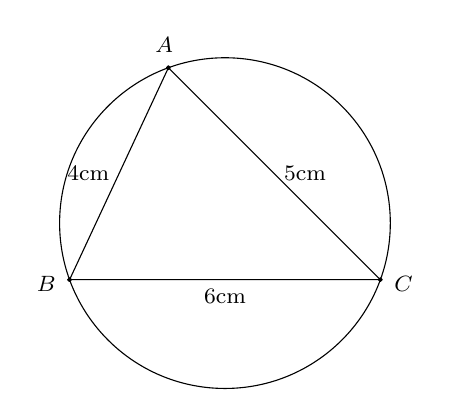
\begin{tikzpicture}[scale=0.7,font=\footnotesize,line join=round,line cap=round,>=stealth]
		\def\r{3} 
		\path 
			(0:0)  coordinate (O)
			(110:\r)  coordinate (A)
			(200:\r) coordinate  (B)
			(-20:\r) coordinate (C); 
		 \draw
			(O)  circle (\r)
			(A)--(B)  node[left,pos=0.5]{$4$cm}--(C) node[below,pos=0.5]{$6$cm}--(A) node[right,pos=0.5]{$5$cm};
		\foreach  \p/\g in {A/100,B/190,C/-10}
		\draw[fill=black]  (\p) circle (1pt) node[shift=(\g:3mm)] {$\p$};
	\end{tikzpicture}
		 }
	\loigiai{ 
		\begin{center}
			\begin{tikzpicture}[scale=0.7,font=\footnotesize,line join=round,line cap=round,>=stealth]
					 \def\r{3}
					\path 
						(0:0) coordinate  (O)
						(110:\r) coordinate (A) 
						 (200:\r) coordinate (B)
						(-20:\r) coordinate  (C)
						 ($(A)!1cm!(B)$) coordinate (b1)
						($(A)!1cm!(C)$) coordinate (c1) 
						($(b1)!0.5!(c1)$) coordinate (a1) 
						(intersection  of A--a1 and B--C) coordinate (D);
					\draw 
						(O) circle  (\r)
						 (A)--(B)--(C)--(A)--(D);
					\foreach \p/\g in {A/100,B/190,C/-10,D/-90} 
					\draw[fill=black] (\p) circle  (1pt) node[shift=(\g:3mm)] {$\p$};
				\end{tikzpicture}
		\end{center}
		\begin{itemchoice}
			\itemch  Đúng.\\
			Nửa  chu vi của tam giác $ABC$ bằng $p=\dfrac{a+b+c}{2}=\dfrac{4+5+6}{2}=\dfrac{15}{2}\,(\mathrm{cm})$.
			\itemch Sai.\\ 
			Áp dụng công  thức Hê-rông\\
			$S=\sqrt{p(p-a)(p-b)(p-c)}=\sqrt{\dfrac{15}{2}\left(\dfrac{15}{2}-6\right)\left(\dfrac{15}{2}-5\right)\left(\dfrac{15}{2}-4\right)}=\dfrac{15\sqrt{7}}{4}\approx  9{,}921$.
			\itemch  Đúng.\\
			Vì $AB < AC < BC$ nên $\widehat{C}  < \widehat{B} < \widehat{A}$.\\
			Áp dụng hệ quả định lí  cô sin cho tam giác $ABC$ ta có\\
			$\cos A=\dfrac{b^2+c^2-a^2}{2bc}=\dfrac{16+25-36}{2\cdot 4\cdot 5}=\dfrac{1}{8}> 0$, do đó $\widehat{A} <  90^\circ$.\\
			Từ đó ta có tam giác $ABC$  là tam giác nhọn.
			 \itemch Đúng.\\
			Theo tính chất của đường phân giác trong ta có $\dfrac{BD}{DC}=\dfrac{AB}{AC}=\dfrac{4}{5}\Rightarrow\dfrac{BD}{BC}=\dfrac{4}{9}\Rightarrow  BD=\dfrac{4}{9}\cdot 6=\dfrac{8}{3}$.\\
			Áp dụng hệ quả  định lí cô sin cho tam giác $ABC$ ta có
			 \[\cos B=\dfrac{a^2+c^2-b^2}{2ac}=\dfrac{36+16-25}{2\cdot 6\cdot 4}=\dfrac{9}{16}.\]
			Áp  dụng định lí cô sin cho tam giác $ABD$ ta có\\
			$AD^2=AB^2+BD^2-2\cdot AB\cdot BD\cdot\cos  B=4^2+\left(\dfrac{8}{3}\right)^2-2\cdot 4\cdot\dfrac{8}{3}\cdot\dfrac{9}{16}=\dfrac{100}{9}$.\\
			$AD=\dfrac{10}{3}\approx 3{,}333$. 
		\end{itemchoice}
	 }
\end{ex}

% nguồn: MaHoaNH_DungSai_Lop10
\begin{ex}%[0H4B2-2]%[ma:8c163b6c]
	Cho tam giác ABC với $AB = 3$ cm, $BC = 4$ cm, và $\widehat{ABC} =  60^{\circ}$. Mỗi kết quả dưới đây đúng hay sai?
	 \choiceTF
		{\True $S =\dfrac{1}{2} \cdot AB \cdot BC \cdot \sin ABC =  3\sqrt{3}$ cm$^2$}
		{\True  $r=\dfrac{S}{p}=\dfrac{-\sqrt{39}+7\sqrt{3}}{6}$, với $p=\dfrac{AB+BC+AC}{2}$}
		{$R =\dfrac{abc}{4S} = \dfrac{\sqrt{13}}{3}$, với $R$ là bán kính đường tròn ngoại tiếp $\triangle ABC$} 
		 {$h_b=\dfrac{2S}{AC}=\dfrac{6\sqrt{13}}{3}$, với $h_b$ là độ dài đường cao hạ từ $B$}
	 \loigiai{
		\begin{itemchoice}
			\itemch $S =\dfrac{1}{2} \cdot AB \cdot  BC \cdot \sin ABC =\dfrac{1}{2} \cdot 3 \cdot 4 \cdot \sin 60^{\circ} = 3\sqrt{3}$ cm$^2$.
			 \itemch
			\begin{itemize}
				\item $AC = \sqrt{AB^2 +  BC^2 - 2 \cdot AB \cdot BC \cdot \cos ABC}=\sqrt{13}$.
				\item $r=\dfrac{S}{p} = \dfrac{AB \cdot BC \cdot  \sin ABC}{AB+BC+CA}=\dfrac{-\sqrt{39}+7\sqrt{3}}{6}$.
			\end{itemize}
			\itemch  $R =\dfrac{abc}{4S}=\dfrac{AB}{2 \sin ABC}=\dfrac{\sqrt{39}}{3}$.
			\itemch $h_b\cdot AC =AB\cdot BC\sin ABC\Rightarrow  h_b= \dfrac{AB\cdot BC\sin ABC}{AC}=\dfrac{6\sqrt{39}}{13}$.
		\end{itemchoice}
	} 
\end{ex}


%%%%%%%%%%%%%%%% TRẢ LỜI NGẮN %%%%%%%%%%%%%%%%

% nguồn: MaHoaNH_TraLoiNgan_Lop10
\begin{bt}%[0H4H2-2]%[ma:c97eee75]
	Cho $\triangle ABC$ có $ BC=a$, $AC=b$. Tam giác $ABC$ có diện tích  lớn nhất khi $\widehat C$ bằng (đơn vị độ)
	 \shortans{90}
	\loigiai{ 
		$S_{ABC}=\dfrac{1}{2}\cdot AC\cdot BC\cdot\sin C=\dfrac{1}{2}\cdot a\cdot b\cdot\sin  C$.\\
	Diện tích tam giác $ ABC$ lớn nhất khi $\sin C$ lớn nhất $\Rightarrow\sin C=1\Leftrightarrow  \widehat{C}=90^\circ$.}
\end{bt}

% nguồn: MaHoaNH_TraLoiNgan_Lop10
\begin{bt}%[0H4H2-2]%[ma:8bccfeeb]
	Cho $\triangle ABC$ có $AB=8$, $AC=5$, $\widehat{BAC}=60^\circ$. Tính  chiều cao $ AH$ của $\triangle ABC$ (làm tròn kết quả đến hàng phần trăm).
	\shortans{4,95} 
	\loigiai{ 
		 $ BC=\sqrt{A{B^2}+A{C^2}-2AB\cdot AC\cdot\cos{60^\circ}}=7$;\\
		${S_{\Delta ABC}}=\dfrac{1}{2}AB\cdot AC\cdot\sin\widehat{BAC}=10\sqrt 3  $.\\
	$S_{\triangle  ABC}=\dfrac{1}{2}AH\cdot BC\Leftrightarrow 10\sqrt 3=\dfrac{1}{2}\cdot 7\cdot AH\Leftrightarrow AH=\dfrac{20\sqrt 3}{7}\approx 4{,}95$.}
\end{bt}

% nguồn: MaHoaNH_TraLoiNgan_Lop10
\begin{bt}%[0H4V2-2]%[ma:cbaef06f]
	Cho tam giác $ABC$ có $\widehat{B}=60^\circ$, $\widehat{A}=30^\circ$, cạnh $BC=12$. Bán  kính đường tròn nội tiếp tam giác $ABC$ là bao nhiêu? (làm tròn kết quả đến hàng phần chục).
	\shortans{4,4} 
	 \loigiai{
		\begin{center}
			\begin{tikzpicture}[scale=0.8,font=\footnotesize,line join = round,line cap = round,>=stealth]
					 \def\r{3}
					\path  (180:\r) coordinate (B)
						(0:\r) coordinate  (C)
						 (130:\r) coordinate (A);
					\draw  (A)--(B)--(C)--cycle
						 pic[draw,angle radius=2mm]{right angle=B--A--C};
					\foreach  \x/ \goc in {A/135,B/-135,C/-45}
					\fill (\x) circle  (1pt)
						($(\x)+(\goc:3mm)$) node {$\x$}; 
				\end{tikzpicture}
		\end{center}
		 Ta có $AC=BC\cdot\tan B\Leftrightarrow AC=12\cdot\tan 60^\circ=12\sqrt{3}$.\\
		$S_{\triangle ABC}=\dfrac{1}{2}\cdot  BC\cdot AC=\dfrac{1}{2}\cdot12\cdot12\sqrt{3}=72\sqrt{3}$.\\
		Áp dụng định lý Pi-ta-go ta được $AB=\sqrt{BC^2+AC^2}=\sqrt{12^2+\left(12\sqrt{3} \right)^2}=24$.\\ 
		Nửa chu  vi tam giác $p=\dfrac{24+12+12\sqrt{3}}{2}=18+6\sqrt{3}$.\\
	 Mà $S_{\triangle ABC}=72\sqrt{3}=p\cdot r\Rightarrow r=\dfrac{S_{\triangle ABC}}{p} \approx 4{,}4$.}
\end{bt}


%%%%%%%%%%%%%%%% TỰ LUẬN %%%%%%%%%%%%%%%%

% nguồn: MaHoaNH_TuLuan_Lop10
\begin{bt}%[0H4H2-2]%[ma:ff89c2dc]
	Cho tam giác nhọn $ ABC$ có $ a=3$, $b=4$ và diện tích $  S=3\sqrt 3 $. Tính bán kính $ R$ của đường tròn ngoại tiếp tam giác đó (làm tròn kết quả đến hàng phầm trăm).
	 \loigiai{
		Ta có $ S=\dfrac{1}{2}ab\sin C\Rightarrow\sin C=\dfrac{2S}{ab}=\dfrac{2\cdot 3\sqrt 3}{3\cdot  4}=\dfrac{\sqrt 3}{2}\Rightarrow\widehat C=60^\circ$.\\
	Theo định lý côsinta có $ c=\sqrt{a^2+b^2-2ab\cos C}=\sqrt{13}$.\\ Theo định lý sinta có$\dfrac{c}{\sin C}=2R\Rightarrow R=\dfrac{c}{2\sin  C}=\dfrac{\sqrt{13}}{2\sin{60^\circ}}=\dfrac{\sqrt{39}}{3}\approx 2{,}08$.}
\end{bt}

% nguồn: MaHoaNH_TuLuan_Lop10
\begin{bt}%[0H4H2-2]%[ma:a00c89ce]
	Cho tam giác $ ABC$ có $BC=a$, $CA=b$, $AB=c$ và $h_a$ là đường cao kẻ từ đỉnh $A$ của tam giác $ ABC$.  Chứng minh rằng $h_a=2R\sin B\sin C$ với $R$ là bán kính đường tròn ngoại tiếp tam giác $ABC$.
	 \loigiai{
		Ta có $S=\dfrac{1}{2}a\cdot{h_a}=\dfrac{1}{2}bc\sin A 
		 \Rightarrow{h_a}=\dfrac{bc\sin A}{a}$.\\
		Theo định lí sinta có $b=2R\sin B$; $c=2R\sin C$ và $\dfrac{\sin A}{a}=\dfrac{1}{2R}$.\\ 
		Khi  đó $h_a=\dfrac{2R\sin B\cdot 2R\sin C\cdot\sin A}{a}=2R\sin B\sin C$.
	} 
\end{bt}

% nguồn: MaHoaNH_TuLuan_Lop10
\begin{bt}%[0H4H2-2]%[ma:bf05cb3a]
	Cho tam giác $ ABC$ biết $ b=7$, $c=5$, $\cos  A=\dfrac{3}{5}$. Tính diện tích tam giác $ABC$ và bán kính đường tròn nội tiếp tam giác $ABC$.
	 \loigiai{
		Ta có $\sin ^2A=1-\cos ^2A=\dfrac{16}{25}\Rightarrow\sin  A=\dfrac{4}{5}$ (vì $\sin A > 0$).\\
		Khi đó diện tích  tam giác $ABC$ là $ S=\dfrac{1}{2}bc\sin A=14$.\\
		 Áp dụng định lý côsin vào tam giác $ABC$, ta có
		\begin{itemize}
			\item $a^2=b^2+c^2-2bc\cos A=7^2+5^2-2\cdot7\cdot  5\cdot\dfrac{3}{5}=32\Rightarrow a=4\sqrt 2 $.
			\item $p=\dfrac{a+b+c}{2}=6+2\sqrt 2  $.
			 \item $ S=pr\Rightarrow r=\dfrac{S}{p}=\dfrac{14}{6+2\sqrt 2}=3-\sqrt 2 $.
		\end{itemize}
	} 
\end{bt}

% nguồn: MaHoaNH_TuLuan_Lop10
\begin{bt}%[0H4V2-2]%[ma:8b34a15c]
	Cho tam giác $ABC$ có hai trung tuyến $BM$  và $CN$ hợp với nhau một góc $120^{\circ}$. Biết $BM=12$, $CN=15$. Tính chu vi của tam giác $ABC$ (kết quả là tròn đến hàng đơn vị).
	\begin{center}
		\begin{tikzpicture}[declare function={a = 5; goc = 65; b = 0.65*a;}]
				 \path
					 (goc:b) coordinate (A)
					(0,0) coordinate (B) 
					(a,0) coordinate (C); 
				\path (barycentric cs:A=1,B=1,C=1)  coordinate (G);
				\path  ($(A)!0.5!(B)$) coordinate (N);
				 \path ($(A)!0.5!(C)$) coordinate (M);
				\foreach \x/\y/\z in {B/G/C}{ 
					\path (\y) pic[draw,angle  radius=20pt,angle eccentricity=0.5,"$120^\circ$"]{angle = \x--\y--\z};
				 }
				\draw (A)--(B)--(C)--cycle; 
				\draw  (M)--(B)
					 (C)--(N);
				\foreach  \t/\g in {A/90,B/-90,C/-90,M/60,N/120,G/90}{
					\draw[fill=white] (\t) circle (1pt) node[shift={(\g:7pt)},font=\scriptsize]{$  \t $};
				} 
			\end{tikzpicture}
	\end{center}
	\loigiai{ 
		\begin{itemize}
			\item Gọi $BM\cap CN=G \Rightarrow G$ là trọng tâm  của tam giác $ABC$.
			\[\Rightarrow GB=\dfrac{2}{3}  BM=8,~ GC=\dfrac{2}{3} CN=10\Rightarrow GM=4,~ GN=5.\]
			Áp dụng  định lý cos trong tam giác $GBC$ có
			\[BC^2=GB^2+GC^2-2GB\cdot GC\cdot \cos 120^{\circ}=244\Rightarrow BC=2\sqrt{61}.\] 
			\item  Ta có $\widehat{BGN}=180^{\circ}-\widehat{BGC}=60^{\circ}$, $\widehat{MGC}=180^{\circ}-\widehat{BGC}=60^{\circ}$.\\
			Áp dụng định lý côsin,  ta được
			\[BN^2=GB^2+GN^2-2GB\cdot GN\cdot \cos 60^{\circ}=49\Rightarrow BN=7\Rightarrow  AB=2BN=14.\]
			\[MC^2=GM^2+GC^2-2GM\cdot GC\cdot \cos 60^{\circ}=76\Rightarrow MC=2\sqrt{19} \Rightarrow  AC=2MC=4\sqrt{19}.\]
		\end{itemize}
		Vậy chu vi của  tam giác $ABC$ là $AB+BC+CA=14+2\sqrt{61}+4\sqrt{19}=47{,}06\approx 47$.
	} 
\end{bt}

% nguồn: MaHoaNH_TuLuan_Lop10
\begin{bt}%[0H4C2-2]%[ma:81cd6d13]
	 \immini[thm]
	 {
	Cho hình vẽ bên, với $M$ là điểm bên trong tam giác sao cho $\widehat{AMB}=\widehat{BMC}=\widehat{CMA}=120^{\circ}$. Đặt $MA=x$,  $MB=y$, $MC=z$. Biết các số thực dương $x$, $y$, $z$ thỏa mãn hệ phương trình $\heva{&x^2+y^2+xy=5 \\& y^2+z^2+yz=6\\ &z^2+x^2+zx=7}$. Tính giá trị biểu thức $S=xy+yz+zx$ (kết quả làm tròn đến hàng phần trăm).
	 }
	{ 
	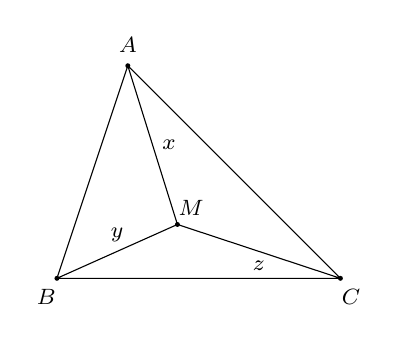
\begin{tikzpicture}[scale=0.9,font=\footnotesize,line join=round,line cap=round,>=stealth]
			 \path
				(2,4) coordinate (A) 
				(1,1) coordinate  (B)
				(5,1)  coordinate (C)
				(2.7,1.76) coordinate (M); 
			\draw (A)--(B)--(C)--(A)--(M)  node[midway,right]{$x$}
				(B)--(M) node[midway,above]{$y$} 
				(M)--(C) node[midway,below]{$z$}; 
			 \foreach \x/\g in {A/90,B/-120,C/-60,M/50}
			\fill[black] (\x)  circle (1pt)+(\g:3mm) node {$\x$};
		\end{tikzpicture}
	 }
	 \loigiai{
		Ta có $AB^2=MA^2+MB^2-2MA\cdot  MB\cdot \cos 120^\circ=x^2+y^2+xy=5\Rightarrow AB=\sqrt{5}$.\\
		Tương tự  ta tính được $BC=\sqrt{6}$, $CA=\sqrt{7}$.\\
		Đặt  $p=\dfrac{AB+BC+AC}{2}=\dfrac{\sqrt{5}+\sqrt{6}+\sqrt{7}}{2}$.\\
		Diện  tích tam giác $ABC$ là $S_{ABC}=\sqrt{p\left(p-AB\right)\left(p-AC\right)\left(p-BC\right)}=\sqrt{\dfrac{13}{2}}$.\\
		Ta có  $S_{AMB}=\dfrac{1}{2}MA \cdot MB\cdot \sin \widehat{AMB}=\dfrac{\sqrt{3}}{4}xy$, $S_{BMC}=\dfrac{\sqrt{3}}{4}yz$, $S_{CMA}=\dfrac{\sqrt{3}}{4}xz$.\\
		 Mà $S_{ABC}=S_{AMB}+S_{BMC}+S_{CMA}=\dfrac{\sqrt{3}}{4}\left(xy+yz+zx\right)$.\\
		Thế nên suy ra $xy+yz+zx=\dfrac{2\sqrt{78}}{3}\approx 5{,}89$. 
	 }
\end{bt}

% nguồn: MaHoaNH_TuLuan_Lop10
\begin{bt}%[0H4B2-2]%[ma:eda16817]
	Viết phương trình đường tròn đường  kính $AB$ với $A(2;3)$, $B(-6;5)$.
	 \loigiai{
		Bán  kính $R=\dfrac{AB}{2}=\dfrac{\sqrt{(-6-2)^2+(5-3)^2}}{2}=\sqrt{17}$.\\
		Tâm $I$ là trung  điểm đoạn $AB$ suy ra $I(-2;4)$.\\
		Phương trình đường tròn đường  kính $AB$ là $$(x+2)^2+(y-4)^2=17.$$
	} 
\end{bt}

% nguồn: MaHoaNH_TuLuan_Lop10
\begin{bt}%[0H4B2-2]%[ma:800fc8ae]
	 (1.0 điểm)
	Viết  phương trình tổng quát của đường tròn có đường kính $A B$ biết $A(-3; 2)$; $B(1; 4)$.
	 \loigiai{
		Tọa độ trung điểm của $  AB $ là $ I(-1;3) $.\\
		Bán kính đường tròn $  R=IA=\sqrt{2^2+1^2}=\sqrt{5} $.\\
		Vậy phương trình đường tròn đường  kính $ AB $ có phương trình là $ (x+1)^2+(y-3)^2=5 $.
	 }
\end{bt}

% nguồn: MaHoaNH_TuLuan_Lop10
\begin{bt}%[0H4Y2-2]%[ma:16acf923]
	Trong mặt phẳng $Oxy$, cho hai điểm $M(3;2)$, $N(1;-4)$. Hãy viết phương trình đường tròn đường  kính $MN$.
	\loigiai{ 
		Gọi $I$ là tâm của  đường tròn. Suy ra, $I$ là trung điểm của $MN$.\\
		 Do đó $I(2;-1)$.\\
		Đường tròn cần  tìm có tâm $I(2;-1)$ và qua $M(3;2)$ có dạng
		$$(x-2)^2+(y+1)^2=(3-2)^2+(2+1)^2  \Leftrightarrow (x-2)^2+(y+1)^2=10.$$
	} 
\end{bt}

% nguồn: MaHoaNH_TuLuan_Lop10
\begin{bt}%[0H4B2-2]%[0H4B2-4]%[0X1Y3-2]%[0X1B4-3]%[ma:cd902c0c]
	 Trong mặt phẳng $Oxy$, viết phương trình đường tròn có tâm $I(3;5)$ và tiếp xúc với đường thẳng $\Delta$ có phương trình $4x + 3y + 23 = 0$.
	\loigiai{ 
		Gọi  $(C)$ là đường tròn cần tìm.\\
		Vì $(C)$ có tâm $I(3;5)$ và tiếp xúc với đường  thẳng $\Delta$ có phương trình $4x + 3y + 23 = 0$ nên bán kính đường tròn $(C)$ chính là khoảng cách từ $I$ đến $\Delta$. Do đó
		$$ R = \mathrm{d}(I,\Delta) = \dfrac{|4\cdot 3 + 3\cdot 5  + 23|}{\sqrt{4^2 + 3^2}} = \dfrac{50}{5} = 10. $$
		Phương trình đường tròn  có tâm $I(3;5)$ và bán kính $R = 10$ là
		$$ (C)\colon (x-3)^2 + (y-5)^2  = 100. $$
	 }
\end{bt}

% nguồn: MaHoaNH_TuLuan_Lop10
\begin{bt}%[0H4B2-2]%[ma:34a60afb]
	Trong mặt phẳng tọa độ $Oxy$, viết phương trình đường tròn $(C)$,  biết
	\begin{enumerate}
		\item $(C)$ có tâm $I(3;-4)$  bán kính $R=\sqrt{3}$.
		\item $(C)$ có tâm $I(3;-4)$ và tiếp xúc với đường thẳng $(\Delta)\colon  x-2y-6=0$.
	\end{enumerate}
	\loigiai{ 
		\begin{enumerate}
			\item Phương  trình đường tròn $(C)$ có tâm $I(3;-4)$ bán kính $R=\sqrt{3}$ là
			 \[(C)\colon (x-3)^2+(y+4)^2=3. \]
			\item Vì $(C)$ tiếp xúc với  đường thẳng $(\Delta)\colon x-2y-6=0$ nên
			\[R=\mathrm{d}(I, \Delta)=\dfrac{|3+8-6|}{\sqrt{5}}=\sqrt{5}.  \]
			Do đó  phương trình đường tròn $(C)$ có tâm $I(3;-4)$ bán kính $R=\sqrt{5}$ là
			\[(C)\colon  (x-3)^2+(y+4)^2=5. \]
		\end{enumerate}
	 }
\end{bt}

% nguồn: MaHoaNH_TuLuan_Lop10
\begin{bt}%[0H4B2-2]%[0H4B1-2]%[ma:5d575813]
	Trong mặt  phẳng tọa độ $Oxy$, cho điểm $A(-1;2)$ và $B(3;-4)$.
	\begin{listEX}
		\item Viết phương trình tổng quát  của đường thẳng $AB$.
		\item Viết phương trình đường  tròn $(C)$ có đường kính $AB$.
	\end{listEX}
	\loigiai{ 
		\begin{listEX}
			\item Đường thẳng $AB$ đi qua $A(-1;2)$ và  $B(3;-4)$ nên nhận $\vec{AB}=(4;-6)$ làm véc-tơ chỉ phương.\\
			Suy ra $AB$ nhận $\vec{n}=(3;2)$ làm một véc-tơ pháp tuyến.\\ 
			Phương trình tổng quát của $AB\colon  3(x+1)+2(y-2)=0 \Leftrightarrow 3x+2y-1=0$.
			 \item Gọi $I$ là trung điểm của $AB$ thì $I(1;-1)$ là tâm của đường tròn $(C)$ đường kính $AB$.\\
			Và $(C)$ có  bán kính $R=IB=\sqrt{(3-1)^2+(-4+1)^2}=\sqrt{13}$.\\
			Phương trình đường tròn đường kính $AB$ là $(C)\colon  (x-1)^2+(y+1)^2=13$.
		\end{listEX}
	} 
\end{bt}

% nguồn: MaHoaNH_TuLuan_Lop10
\begin{bt}%[0H4K2-2]%[ma:b8503e98]
	Viết phương trình đường tròn $(C)$ có bán kính $R=2$, tâm $I$ thuộc đường thẳng $\Delta_1\colon \left\{\begin{aligned}
	 & x=1+t\\ & y=1-t\\
\end{aligned}\right.$ và $(C)$ tiếp xúc với đường thẳng $\Delta_2\colon 3x+4y-1=0$.
 \loigiai{
	Theo đề $I\in \Delta_1\Rightarrow  I(1+t;1-t)$.\\
	Vì $(C)$ tiếp xúc với đường thẳng $\Delta_2$ và có bán  kính $R=2$ nên ta có\\
	\allowdisplaybreaks \vspace*{-0.7cm} 
	\begin{eqnarray*}
		& R= &\mathrm{d}(I,\Delta_2)=2\\ 
		& \Leftrightarrow &  \dfrac{\left| 3(1+t)+4(1-t)-1\right|}{\sqrt{3^2+4^2}}=2\\
		& \Leftrightarrow &  \left| 6-t\right|=10\\
		& \Leftrightarrow & \left[\begin{aligned}
		& t=-4\\ &  t=16.\\
	\end{aligned}\right.
	\end{eqnarray*}
	Với $t=-4\Rightarrow I\left(-3;5\right)$; 
	 và $t=16\Rightarrow I\left(17;-15\right)$.\\
	Vậy có hai đường tròn $(C)$  cần tìm là:\\ $\left(x+3\right)^2+\left(y-5\right)^2=4$
	 hoặc $\left(x-17\right)^2+\left(y+15\right)^2=4$.
 }
\end{bt}

% nguồn: MaHoaNH_TuLuan_Lop10
\begin{bt}%[0H4B2-2]%[0H4B2-3]%[ma:10f472ea]
	Trong mặt phẳng tọa độ $Oxy$, cho  ba điểm $A(4;0)$, $B(0;3)$, $C(2;4)$.
	\begin{enumerate}
		\item Viết phương trình tổng  quát của đường thẳng $AB$.
		 \item Viết phương trình đường tròn $(T)$ tâm $C$ và tiếp xúc với đường thẳng $AB$.
		\item Một điểm có cả hoành độ và tung độ là số nguyên được gọi là điểm nguyên. Biết rằng trên đường tròn $(T)$ có bốn điểm nguyên. Bốn điểm này là bốn  đỉnh của một tứ giác lồi. Tính diện tích của tứ giác lồi đó.
	\end{enumerate}
	 \loigiai{
		\begin{enumerate}
			\item Ta có  $\overrightarrow{AB}=(-4;3)$ là một véc-tơ chỉ phương của đường thẳng $AB$.\\
			Suy ra $\overrightarrow{n}=(3;4)$ là một véc-tơ pháp tuyến  của đường thẳng $AB$.\\
			Đường thẳng $AB$ đi qua $A(4;0)$, có một véc-tơ pháp tuyến $\overrightarrow{n}=(3;4)$ nên có  phương trình là \[3(x-4)+4(y-0)=0 \Leftrightarrow 3 x+4 y-12=0.\]
			{\bf Cách khác.} Ta có phương trình đường thẳng $AB$ theo đoạn chắn là $\dfrac{x}{4}+\dfrac{y}{3}=1\Leftrightarrow 3x+4y-12=0$. 
			\item Đường tròn  $(T)$ tâm $C(2;4)$ và tiếp xúc với đường thẳng $AB$ nên có bán kính là
			\[R=\mathrm{d}  (C, AB)=\dfrac{|3 \cdot 2+4 \cdot 4-12|}{\sqrt{3^2+4^2}}=2.\]
			Vậy  $(T)$ có phương trình là $(x-2)^2+(y-4)^2=4$.
			\item Số $4$ được phân tích thành tổng của hai số chính phương là $4=0+4=4+0$.\\ 
			Với  $(x-2)^2+(y-4)^2=4$ và $x$, $y \in \mathbb{Z}$ ta có
			\[\heva{&(x-2)^2=0\\&(y-4)^2=4} 
			\Leftrightarrow \heva{&x=2\\&y=6}\text{ hoặc  } \heva{&x=2\\&y=2.}\]
			\[ 
			 \heva{&(x-2)^2=4\\&(y-4)^2=0}
			\Leftrightarrow \heva{&x=0\\&y=4}\text{ hoặc }  \heva{&x=4\\&y=4.}
			\] 
			Trên $T$ có bốn điểm nguyên  là $M(0;4)$, $N(2;6)$, $P(4;4)$, $Q(2;2)$.\\
			Dễ thấy $MNPQ$ là hình vuông có đường chéo  $MP=NQ=4$. \\
			Diện tích hình  vuông $MNPQ$ là $S=\dfrac{1}{2}\cdot 4^2=8$ (đơn vị diện tích).
		\end{enumerate}
	 }
\end{bt}
